\chapter{Конструкторская часть}
В данном разделе представлена схема, поясняющая принцип рабо­ты
алгоритма конвейерной обработки данных, а также схема алгоритма 
поставленной задачи.

\section{Схемы работы алгоритма конвейерной обработки данных}

На рисунке \ref{pic:schema-pipeline} представлена схема, поясняющая принцип работы
конвейерной обработки данных.

\begin{figure}[!htb]
	\centering
	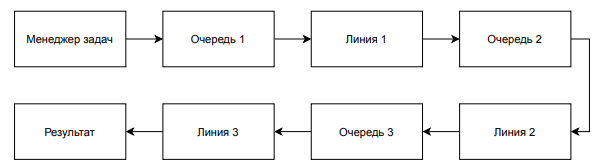
\includegraphics[scale=0.55]{imgs/3}
	\caption{Схема, иллюстрирующая пример работы конвейра с
	параллельной реализацией}
	\label{pic:schema-pipeline}
\end{figure}


Заметим, что вычисление хеш-суммы файла не зависит от ранее вычисленных
значений. В связи с этим, можно реализовать многопоточное вычисление хеш-сумм файлов,
посредством так называемых fan-out и fan-in подходов.

Таким образом, получим схему работы конвейера, отраженную на рисунке \ref{pic:schema-fanin-fanout}.
\begin{figure}[!htb]
	\centering
	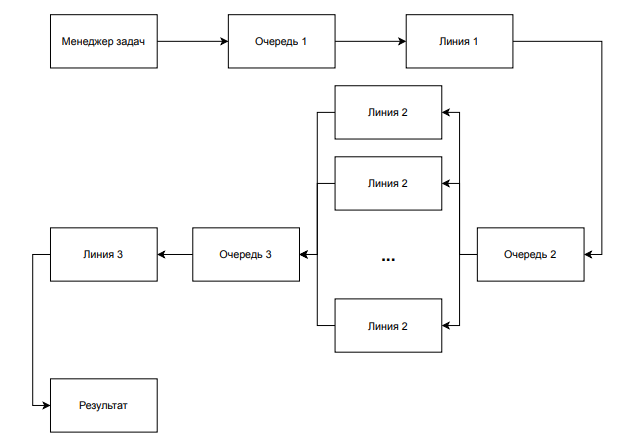
\includegraphics[scale=0.55]{imgs/4}
	\caption{Схема организации конвейерных вычислений fan-in/fan-out}
	\label{pic:schema-fanin-fanout}
\end{figure}


Отдельно стоит отметить, что в алгоритме, рассматриваемом в рамках данной лабораторной работы,
используется, по сути, статический менеджер задач, поскольку все задачи - это файлы в указанной директории.


\section{Описание структуры программного обеспечения}

Программа будет включать в себя один смысловой модуль, на­
зываемый \code{md5pipeline}, который содержит в себе процедуры и функции,
связанные с реализацией параллельного и синхронного конвейера. Неза­
висимо от модуля будет существовать файл \code{main.go}, одержащий точку входа в программу,
а так же \code{handling.go}, в котором будет реализован подсчет	статистики.

Программа разбита на модули:
\begin{itemize}
	\item \code{main.go} - файл, содержащий точку входа в программу;
	\item \code{handling.go} - файл, содержащий реализацию подсчета статистики;
	\item \code{md5pipeline/types.go} - определение пользовательских типов даных;
	\item \code{md5pipeline/pipeline.go} - определение структуры конвейера;
	\item \code{md5pipeline/filescanner.go} - реализация первой ленты конвейера;
	\item \code{md5pipeline/digester.go} - реализация второй ленты конвейера;
	\item \code{md5pipeline/md5.go} - реализация третьей ленты конвейера;
\end{itemize}

На Рисунке \ref{pic:idef0} представлена idef0–диаграмма работы описанного выше конвейера.
\begin{figure}[!htb]
	\centering
	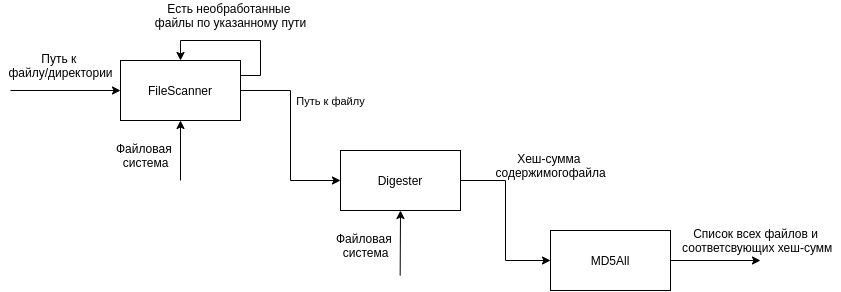
\includegraphics[scale=0.55]{imgs/5}
	\caption{Диаграмма работы конвейера}
	\label{pic:idef0}
\end{figure}


\section{Описание структур данных}

Для реализации конвейерных вычислений, введем некоторые типы данных:
\begin{itemize}
	\item \texttt{FileScannerOutput} – структура, описывающая результат обработки задачи первой лентой конвейера;
	\item \texttt{DigesterOutput} – структура, описывающая результат обработки задачи второй лентой конвейера;
	\item \texttt{ResultingOutput} – структура, описывающая результат обработки задачи конвейером.
\end{itemize}

Рассмотрим каждый из введенных типов данных

\begin{lstlisting}[label=lst:fsOutput,caption={Определение типов данных. FileScannerOutput}]
type fileScannerOutput struct {
	path string

	startTime        time.Time
	endTime          time.Time
\end{lstlisting}

На листинге \ref{lst:fsOutput}:
\begin{itemize}
	\item \texttt{path} - путь, к рассматриваемому файлу/директории;
	\item \texttt{startTime} - время начала обработки задачи первой лентой;
	\item \texttt{endTime} - время постановки задачи в очередь.
\end{itemize}


\begin{lstlisting}[label=lst:dOutput,caption={Определение типов данных. DigesterOutput}]
type digesterOutput struct {
	path string
	sum  [md5.Size]byte
	err  error

	startFileScannerTime time.Time
	endFileScannerTime   time.Time

	waitingTimeInQueue time.Duration
	startTime        time.Time
	queuingTime      time.Time
}
\end{lstlisting}
	
На листинге \ref{lst:dOutput}:
\begin{itemize}
	\item \texttt{path} - путь, к рассматриваемому файлу/директории;
	\item \texttt{sum} - хеш-сумма содержимого файла;
	\item \texttt{err} - поле, содержащее описание ошибки обработки задачи, при наличии таковой;\
	
	\item \code{startFileScannerTime} - время начала обработки задачи первой лентой;
	\item \code{endFileScannerTime} - время окончания обработки задачи первой лентой;

	\item \code{waitingTimeInQueue} - длительность простоя задачи перед второй лентой;
	\item \texttt{startTime} - время начала обработки задачи второй лентой;
	\item \texttt{queuingTime} - время постановки задачи в очередь.
\end{itemize}
	

\begin{lstlisting}[label=lst:resOutput,caption={Определение типов данных. ResultingOutput}]
type ResultingOutput struct {
	Path string
	Sum  [md5.Size]byte

	Start1              time.Time
	End1                time.Time

	WaitingForDigester time.Duration
	Start2           time.Time
	End2             time.Time

	WaitingForAggregation time.Duration
	Start3              time.Time
	End3                time.Time
}
\end{lstlisting}
	
На листинге \ref{lst:resOutput}:
\begin{itemize}
	\item \texttt{Path} - путь, к рассматриваемому файлу/директории;
	\item \texttt{Sum} - хеш-сумма содержимого файла;
	
	\item \code{Start1} - время начала обработки задачи первой лентой;
	\item \code{End1} - время окончания обработки задачи первой лентой;

	\item \code{WaitWaitingForDigester} - длительность простоя задачи перед второй лентой;
	\item \code{Start2} - время начала обработки задачи второй лентой;
	\item \code{End2} - время окончания обработки задачи второй лентой;

	\item \code{WaitingForAggregation} - длительность простоя задачи перед третьей лентой;
	\item \code{Start3} - время начала обработки задачи третьей лентой;
	\item \code{End3} - время окончания обработки задачи третьей лентой;
\end{itemize}


\section{Вывод}
На основе теоретических данных, полученных из аналитического раздела, была построена схема
организации конвейерных вычислений на примере конвейере с тремя лентами (Рисунок \ref{pic:schema-pipeline}).
Так же, было приведено описание пользовательских типов данных, описанных в рамках
реализации конвейерных вычислений (Листинги \ref{lst:fsOutput} -- \ref{lst:resOutput})